% created on 30/03/2020
% @author : ebazan
\part{Image Texture}
\chapter{Spectral Descomposition of an Image}
\section{Texure Imformation in Image Analysis}

\section{The Gabor filter as a measurement tool}\label{ch:gabor_filter_description}

In this chapter we present a reminder of the signal theory applied to image processing for feature extraction and object detection. First, we show what are the reasons for restricting signal analysis in two predefined domains: time and frequency in one dimension and space and frequency in two dimensions. We especially recall Gabor's filter theory and properties by showing how these filters are related to Heisneberg's uncertainty principle.

As we mentioned before, we use Gabor filters as a tool to measure the information that characterizes a signal. Since the signal information can relevant information at different points and scales (either in the spatial or space-frequency domain), a well-known strategy used in the literature is to create a filter bank that covers most of the spectrum to be able to reconstruct the original signal.

\subsection{Signals in two domains}

In the area of signal and image processing it is well known that there are two alternative methods for describing signals (one-dimensional (1-d) or two-dimensional (2-d)). The first one is to represent the signal as a function of time while the second is to represent the signal as a function of frequency. These two representations are of special interest because we can go from one to the other via the Fourier transform (or the inverse Fourier transform); therefore, these two representations carry the same signal information but in different ways. In this thesis the following Fourier transforms pairs are used

\begin{equation}\label{eq:fourier_transforms_1d}
    \begin{gathered}
        H(\upsilon) = \mathcal{F}\{h(t)\} = \int_{-\infty}^{\infty} h(t) e^{-j2\pi f t} dt \\
        h(t) = \mathcal{F}^{-1}\{H(\upsilon)\} = \int_{-\infty}^{\infty} H(\upsilon) e^{j2\pi f t} df 
    \end{gathered}
\end{equation}

for a 1-d space and 

\begin{equation}\label{eq:fourier_transforms_2d}
    \begin{gathered}
        H(u, v) = \mathcal{F}\{h(x, y)\} = \int_{-\infty}^{\infty} \int_{-\infty}^{\infty} h(x, y) e^{-j2\pi (ux + vy)} dx dy \\
        h(x, y) = \mathcal{F}^{-1}\{H(u, v)\} = \int_{-\infty}^{\infty} \int_{-\infty}^{\infty}  H(u, v) e^{j2\pi (ux + vy)} du dv 
    \end{gathered}
\end{equation}

for a 2-d space. Both representations of the signal are somewhat ideal, since the first operates at defined instants of time while the second operates on an infinite series of successive waves at defined frequencies \cite{Gabor:JIEE:1946a}. 

It is evident that the function $h(t)$ is located in both domains, however, it is also well known that no signal with compact support cannot have a finite Fourier transform and vice versa \cite{Bracewell:FourierBook:1999}, there is a certain uncertainty in the time and frequency locations of $h(t)$.

\subsection{The Heisenberg uncertainty principle }

The uncertainty principle is one of the most famous ideas in quantum mechanics. An early incarnation of the uncertainty principle appeared in a 1927 paper by the German physicist Heisenberg. The uncertainty principle says that we cannot measure the position $(x)$ and the momentum $(p)$ of a particle with absolute precision. The more accurately we know one of these values, the less accurately we know the other. 

However, the uncertainty principle in the field of quantum mechanics is just a particular case of a more general compromise that appears in simple phenomena of everyday life involving waves. The central idea is connected with the interrelation between frequency and duration. For example, in the case of sound waves, if we want to identify the frequency of a musical note, the shorter the sound lasts in time, the less certain we can be about the exact frequency of the sound; to find a more defined frequency, it would be necessary to listen to the sound for a longer time. In the language of signal processing, we can say that a short signal correlates highly with a wide range of frequencies and only wide signals correlate with a short range of frequencies. Formally this is expressed as

\begin{equation}\label{eq:uncertainty_principle_rad}
	\Delta t\Delta \omega \geq \frac{1}{2}
\end{equation}

where $\Delta t$ is the duration of the signal in the time domain and $\Delta \omega$ is the bandwidth of the signal in the frequency domain (CITE). The uncertainty principle then says: the product of the spectral bandwidth multiplied with the time duration of the signal cannot be less than a certain minimum value. Considering the bandwidth of the signal in terms of frequency as $\Delta \upsilon$ where $\omega = 2\pi \upsilon$, the uncertainty principle is stated as 

\begin{equation}\label{eq:uncertainty_principle_freq}
	\Delta t\Delta \upsilon \geq \frac{1}{4\pi}
\end{equation}

The Heisenberg uncertainty principle in the field of signal processing and image processing can be mathematically proved by the \textbf{Parseval's theorem}

\begin{equation}\label{eq:parseval_theorem}
	\int_{-\infty}^{\infty} h(t)^2 dt =  \frac{1}{2 \pi} \int_{-\infty}^{\infty} |H(\omega)|^2 d\omega =  \int_{-\infty}^{\infty} |H(\upsilon)|^2 d\upsilon
\end{equation}

where $h(t)$ is a function and $H(\upsilon)$ its the Fourier transform. 

The \textbf{energy content} of the signal described by $h(t)$ is defined as:

\begin{equation}\label{eq:energy_content_time}
    E_{\infty} \equiv \int_{-\infty}^{\infty}  h(t)^2 dt
\end{equation}


From the Parseval's identity this may be written as:

\begin{equation}\label{eq:energy_content_frequency}
    E_{\infty} =  \int_{-\infty}^{\infty} |H(\upsilon)|^2 d\upsilon
\end{equation}

The \textbf{time dispersion} of the signal is given by

\begin{equation}\label{eq:time_dispersion_no_centered}
    (\Delta t)^2 \equiv \frac{1}{E_{\infty}} \int_{-\infty}^{\infty} (t-t_{0})^2 h(t)^2 dt
\end{equation}

where $t_0$ is the \textbf{center of gravity} of the signal defined by:

\begin{equation}\label{eq:center_of_gravity}
    t_0 \equiv \frac{1}{E_{\infty}} \int_{-\infty}^{\infty} t h(t)^2 dt
\end{equation}

and where if we shift the origin of $t$ so that $t_{0}=0$, then

\begin{equation}\label{eq:time_dispersion}
    (\Delta t)^2 = \frac{1}{E_{\infty}} \int_{-\infty}^{\infty} t^2 h(t)^2 dt
\end{equation}

In an analogous way, the \textbf{spectral bandwidth} of the signal is given by

\begin{equation}\label{eq:spectral_bandwidth_no_centered}
    (\Delta \upsilon)^2 \equiv \frac{1}{E_{\infty}} \int_{-\infty}^{\infty} (\upsilon-f)^2 |H(\upsilon)|^2 d\upsilon
\end{equation}

where $f$ is the \textbf{spectral center of gravity} of the signal defined by:

\begin{equation}\label{eq:spectral_center_of_gravity}
    f \equiv  \frac{2 \pi}{E_{\infty}} \int_{-\infty}^{\infty} f |H(\upsilon)|^2 d\upsilon
\end{equation}

if we consider $f=0$:

\begin{equation}\label{eq:spectral_bandwidth}
    (\Delta \upsilon)^2 = \frac{1}{E_{\infty}} \int_{-\infty}^{\infty} f^2 |H(\upsilon)|^2 d\upsilon 
\end{equation}

If $h'(t)$ is the derivative of the function, its Fourier transform is $j2\pi f H(\upsilon)$. By applying the Parseval's theorem to the Fourier pair $h'(t)\longleftrightarrow j2\pi f H(\upsilon)$ we obtain:

\begin{equation}\label{eq:applyed_parseval_theorem}
    4 \pi^{2} \int_{-\infty}^{\infty} f^2 |H(\upsilon)|^2 d\upsilon =  \int_{-\infty}^{\infty} h'(t)^2 dt
\end{equation}

By substituting in equation $(\eqref{eq:spectral_bandwidth})$, we have:

\begin{equation}\label{eq:spectral_bandwidth2}
    (\Delta \upsilon)^2 = \frac{1}{4 \pi^{2} E_{\infty}} \int_{-\infty}^{\infty} h'(t)^2 dt
\end{equation}

We use equations $(\eqref{eq:time_dispersion})$ and $\eqref{eq:spectral_bandwidth2}$ to calculate:

\begin{equation}\label{eq:time_bandwidth_disp}
    (\Delta t)^2(\Delta \upsilon)^2 = \frac{1}{4 \pi^{2} E_{\infty}^{2}} \int_{-\infty}^{\infty} t^2h(t)^2 dt \int_{-\infty}^{\infty}h'(t)^2 dt
\end{equation}

Applying the Schwartz's inequality for the integrals on the right-hand side of $\eqref{eq:time_bandwidth_disp}$:

\begin{equation}\label{eq:schwartz_inequality}
    \int_{-\infty}^{\infty}t h(t)^2 dt \int_{-\infty}^{\infty}h'(t)^2 dt  \geq \biggr\rvert \int_{-\infty}^{\infty}t h(t)h'(t)^2 dt \biggr\rvert^{2}
\end{equation}

We may integrate by parts the integral on the right-hand side of $\eqref{eq:schwartz_inequality}$

\begin{equation}\label{eq:integr_by_parts}
    \int_{-\infty}^{\infty}t h(t) h'(t)^2 dt =  \frac{1}{2}t h(t)^2 \biggr\rvert_{-\infty}^{\infty} - \frac{1}{2} \int_{-\infty}^{\infty}h(t)^2 dt
\end{equation}

If $\lim_{t\rightarrow \infty} t h(t)^2=0$, the first term on the right-hand side of $\eqref{eq:integr_by_parts}$ vanishes and from equation $\eqref{eq:energy_content_time}$ we have

\begin{equation}\label{eq:energy_content_developped}
    \int_{-\infty}^{\infty} t h(t)h'(t) dt = -\frac{1}{2} E_{\infty}
\end{equation}

If we use this into $\eqref{eq:schwartz_inequality}$ and then into $\eqref{eq:time_bandwidth_disp}$ we obtain:

\begin{equation}\label{eq:uncertainty_principle_freq_square}
   (\Delta t)^2(\Delta \upsilon)^2 \geq \frac{1}{16\pi^{2}} 
\end{equation}

This is the mathematical statement of the uncertainty principle in signal processing.

\subsection{1-d Gabor filters}

The uncertainty principle shows that time and frequency are two fundamental domains and physically measurable quantities, but still idealizations if one is considered from the other's perspective.
Frequency is a simple waveform in the time domain, but to be sharply defined in the frequency domain it must be infinite in the time domain; a waveform always existed and remains forever. In everyday life it is very difficult to find phenomena with these characteristics, it is more common to find signals that have properties from both domains; certainly they have some frequency characteristics, but they also have a starting point and after some time these signals begin to fade away. This was the motivation of Dennis Gabor to represent signals simultaneously in time and frequency through the Gabor Elementary Function (GEF) \cite{Gabor:JIEE:1946a}. The function represents the minimal quantum of information, that is, it occupies the minimal area, a rectangle, in the time-frequency plane; the minimal amount of simultaneous information in time and frequency.  

The Gabor function is derived form the uncertainty principle, therefore, it has shape for which the product $\Delta t \Delta \upsilon$ assumes the smallest possible value, i.e., for which the inequality in \eqref{eq:uncertainty_principle_freq} turns into an equality ($\Delta t \Delta \upsilon = \frac{1}{4 \pi}$). This is the modulation product of a harmonic oscillation of any frequency with pulse of the form of a probability function \cite{Gabor:JIEE:1946a}

\begin{equation}\label{eq:gabor_function_1d_time}
    g(t) =  e ^{-\alpha^2(t-t_0)^2} e ^{j 2 \pi f t + \phi}
\end{equation}

where $\alpha$ express the \textit{spread} and $t_0$ denotes the centroid of the Gaussian function, $f$ is the frequency of the harmonic oscillations, and $\phi$ defines the phase shift of the oscillation. The representation of the Gabor function in the frequency domain is defined by the Fourier transform of \eqref{eq:gabor_function_1d_time} $G(\upsilon) = \mathcal{F}\{g(t)\}$ and has the analytical form

\begin{equation}\label{eq:gabor_function_1d_freq}
    G(\upsilon) =  \sqrt{\frac{\pi}{\alpha^2}} e ^{-\left(\frac{\pi}{\alpha}\right) ^{2} (\upsilon-f)^2} e ^{-j 2 \pi t_0 (\upsilon-f) + \phi}
\end{equation}

The equations \eqref{eq:gabor_function_1d_time} and \eqref{eq:gabor_function_1d_freq} show straightforward that the center of gravity $t_0$ is equal to \eqref{eq:center_of_gravity} and the spectral center of gravity $f$ is equal to \eqref{eq:spectral_center_of_gravity}, i.e., the Gabor functions follow the Heisenberg's uncertainty principle.   


\subsubsection{Filter normalization} \label{subsec:filter_normalization}

The Gabor filter can be more appropriately defined by taking the following justifications. First, we must remember that we use the Gabor function as a linear filter to analyze a signal. Under this condition, the temporal analysis of the signal is carried out using the convolution operator. Considering that the Gabor function is concentrated near the time instant $t_0$ and that a convolution centered at the origin is preferable, then $t_0 = 0$. Another parameter that we can omit is the phase shift $\phi$. There is no evidence that any specific phase would be more beneficial than any other. Moreover, for the functions to be similar at all locations, the phase shift should depend on the location $t_0$, and thus, the phase shift can be removed from the origin centered filter ($\phi$ = 0). The Gabor filter function in its compact form is defined as 

\begin{equation}\label{eq:gabor_function_1d_timefreq_compact}
    \begin{gathered}
         g(t) =  e ^{-\alpha^2 t^2} e ^{j 2 \pi f t } \\
         G(\upsilon) =  \sqrt{\frac{\pi}{\alpha^2}} e ^{-\left(\frac{\pi}{\alpha}\right) ^{2} (\upsilon-f)^2} 
     \end{gathered}
\end{equation}

The normalization of the Gabor filter can be performed taking into account the application in which it will be used. However, in this thesis we use the general normalization which is based on the multi domain representation property of the function and following the next conditions \cite{Boukerroui.Noble.ea:JMIV:2004}:

\begin{enumerate}
    \item Maximum condition:
        \begin{equation}\label{eq:maximun_condition}
            \max{|G(\upsilon)|} = 1
        \end{equation}
    \item Constant spectra condition:
        \begin{equation}\label{eq:constant_spectrum_condition}
            \int_{-\infty}^{\infty} |g(t)| dt = 1
        \end{equation}        
\end{enumerate}

From the equation \eqref{eq:gabor_function_1d_freq}, it is evident that the maximum response of the Gabor filter in the frequency domain is a function of $\sqrt{\pi/\alpha^2}$, therefore, its inverse

\begin{equation}\label{eq:normalization_factor}
    \sqrt{\frac{\alpha^2}{\pi}}
\end{equation}

can be used as the Gabor filter normalization factor in the time domain and fulfill the two conditions mentioned above. In summary, the function of the normalized Gabor filter can be defined as

\begin{equation}\label{eq:gabor_function_1d_timefreq_normalized}
    \begin{gathered}
         g(t) =  \sqrt{\frac{\alpha^2}{\pi}} e ^{-\alpha^2 t^2} e ^{j 2 \pi f t } \\
         G(\upsilon) =  e ^{-\left(\frac{\pi}{\alpha}\right) ^2 (\upsilon-f)^2}
     \end{gathered}
\end{equation}

\begin{figure}
\centering
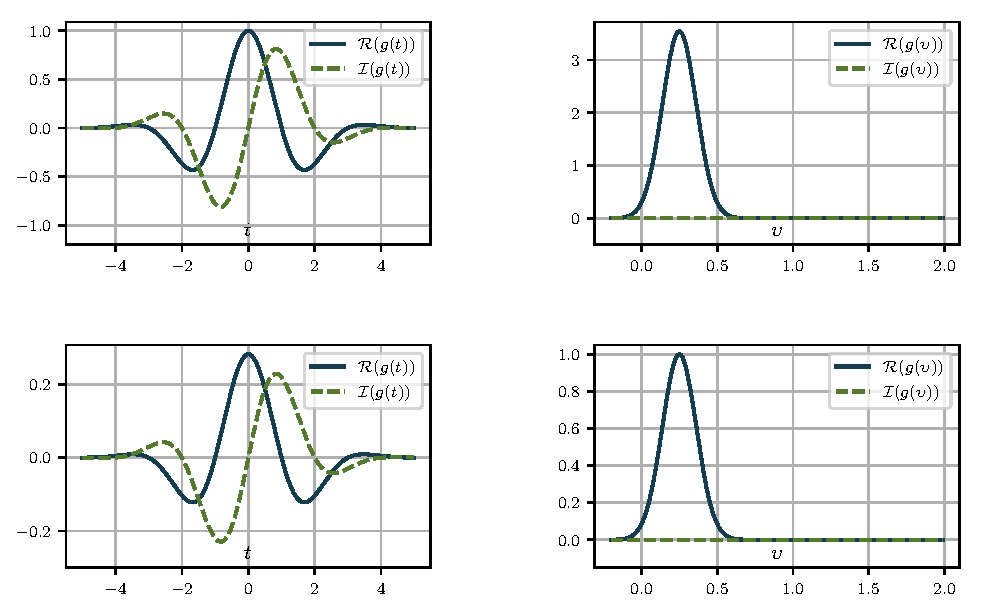
\includegraphics{GaborFilter_timefreq_1d_norm_efect.pdf}
\caption{1-d Gabor filter in the time domain (first column) and in the frequency domain (second  column). From top to bottom: no normalized filter and normalized Gabor filter with $[f =1/4,\alpha=0.5, t_0=0]$.}\label{fig:GaborFilter_timefreq_norm_efect}
\end{figure}

The figure \ref{fig:GaborFilter_timefreq_norm_efect} shows a Gabor filter in the time and frequency domain before and after normalization following the two conditions described above. At this point, it is important to note that normalization is an essential step in the multi-spectral analysis and the feuture extraction of a signal.

\subsubsection{Frequency filter spacing} \label{subsec:frequency_filter_spacing}

Our main interest in Gabor filters is multispectral analysis of a function. To accomplish this, we can generate a bank containing different Gabor functions that work at different frequencies $f$. We can define the separation of the filters in octaves by means of the half-response spatial frequency bandwidth $B_f$ measured between two central frequencies $f_1 < f_2$ \cite{Granlund:CGIP:1978}  

\begin{equation}\label{eq:octave_spacing}
    B_f = \log_2 \left( \frac{f_2}{f_1} \right)
\end{equation}

The octave spacing between two different two adjacent filters is an interesting property of the Gabor filters, however, the filters denoted by the equations \eqref{eq:gabor_function_1d_timefreq_normalized} have a spread that only depends on the parameter $\alpha$, regardless of its central frequency $f$. This means that when implementing the Gabor function in a filter bank at different frequencies to obtain a multi-spectral decomposition of a signal, all of the filters will have the same duration. We can see this effect in Figure \ref{fig:filterbnk_octave_spacing}, where we show a filter bank with an adjacent filter's spacing of one octave, that is, $B_f = 1$. 


\subsubsection{Frequency crossing point}

The fact that the bank filters have the same width at all frequencies is not a problem nor is it a requirement to analyze a signal with the Gabor function, however, making the filter width dependent on its frequency implies a multi-resolution analysis, since the filters behave like a scaled version of each other. One way to accomplish this, is to have the same relative window size in relation to the central frequency $f$. We must remember that window size of a Gabor function is denoted by the effective width of a Gaussian function, which in the time domain has a form of

\begin{equation}\label{eq:1d_gaussian_function_time}
    w(t)=e^{-\frac{(t-t_0)^2}{2\sigma^2}}
\end{equation}

A Gaussian window is infinite in extent, so it is characterized by its locality $t_0$ and its standard deviation $\sigma$, which in this context is implicit in the parameter $\alpha$ of th Gabor fuction, therefore, $\alpha^2 = 1 / 2 \sigma^2$. 
A peculiarity of the Gabor filter is that its analytical form in the frequency domain is completely defined by the fourier transform of the normalized Gaussian function.

\begin{equation}\label{eq:1d_gaussian_function_freq}
    G(\upsilon) = w(\upsilon) = e ^{-\left(\frac{\pi}{\alpha}\right) ^{2} (\upsilon-f)^2}
\end{equation}

Since the center frequencies of the bank filters are chosen to have a constant separation between them and the effective width of the window is a function of this central frequency, there is a point on the frequency axis where two adjacent functions intersect. In a filter bank with two functions with central frequencies $f_1$ and $f_2$, the low cut-off frequency of the function at $f_1$ coincides with the high cut-off frequency of the function at $f_2$. Normally in the literature this crossing point $c_1$, corresponds to the points where the Gabor function has decreased half of its maximum value, i.e., $c_1= 1/2=0.5$ \cite{Granlund:CGIP:1978}. However, we can obtain this crossing point $c_1$ by defining a frequency interval $\Delta f$ that represents the distance between the points where the function $G(\upsilon)$ begins to decrease, therefore, evaluating Eq. \eqref{eq:1d_gaussian_function_freq} at $\upsilon = f + \frac{\Delta f}{2}$

\begin{equation}\label{eq:constant_crossing_point}
    G\left(f + \frac{\Delta f}{2}\right) = e^{-\left(\frac{\pi}{\alpha}\right)^2 \left(\frac{\Delta f}{2}\right)^2} = c_1 G(f) 
\end{equation}

we obtain the expression of the half-frequency interval 

\begin{equation}\label{eq:frequency_interval_crossing_point}
    \frac{\Delta f}{2} = \frac{\alpha}{\pi}\sqrt{\ln \left(\frac{1}{c_1}\right)}
\end{equation}

from which we obtain the crossing point defined as

\begin{equation}\label{eq:crossing_point}
    c_1 = e^{-\left(\frac{\alpha}{\pi} \right)^2 \left(\frac{\Delta f}{2}\right)^2 }
\end{equation}

Then, we know that for a filter whose center frequency is $f$ and whose cut-off frequency interval is $\Delta f$, the full bandwidth expressed in octaves, $B_f$, is defined as \cite{Daugman:JOSA:1985a}

\begin{equation}\label{eq:frequency_bandwidth_interval}
    B_f = \log_2 \left( \frac{f + \frac{\Delta f}{2} }{f - \frac{\Delta f}{2}} \right)
\end{equation}

It is clear that using expression \eqref{eq:frequency_interval_crossing_point} in equation \eqref{eq:frequency_bandwidth_interval}, we find the expression that relates the frequency bandwidth to the central frequency and the effective width of the Gaussian window.

\begin{equation}\label{eq:frequency_bandwidth}
    B_f = \log_2 \left( \frac{ \frac{f}{\alpha} \pi + \sqrt{\ln \left(\frac{1}{c_1}\right)} }{ \frac{f}{\alpha} \pi - \sqrt{\ln \left(\frac{1}{c_1}\right)} } \right)
\end{equation}


The above analysis allows us to rewrite the expression of a Gabor filter in 1-d that belongs to a bank of filters spaced from each other by a bandwidth $B_f$ and a center frequency $f$ as follows. 

\begin{equation}\label{eq:gabor_function_1d_timefreq_bank}
    \begin{gathered}
         g(t) =  \frac{f}{\gamma \sqrt{\pi}} e ^{-\left(\frac{f}{\gamma}\right)^2 t^2} e ^{j 2 \pi f t } \\
         G(\upsilon) =  e ^{-\left(\frac{\gamma \pi}{f}\right) ^2 (\upsilon-f)^2}
     \end{gathered}
\end{equation}
where now the effective bandwidth $\alpha$ of each filter in the bank will be determined based on the ratio $\gamma = \frac{f}{\alpha}$ and crossing point between adjacent filters $c_1$.

The figure \ref{fig:1d_filterbank_spacing} shows the octave spacing for a bank of filters in the frequency domain. Particulary, the figure \ref{fig:filterbnk_octave_spacing} shows a bank without the relationship between the effective width and the central frequency of the filter, whereas the figures \ref{fig:filterbnk_half_crossingpoint} and \ref{fig:filterbnk_new_crossingpoint} show the interdependence between $\alpha$, $B_f$, $f$ and $c_1$ and the behavior of the bank with a different crossing point.

\begin{figure}
\centering
    \subcaptionbox{\label{fig:filterbnk_octave_spacing}}{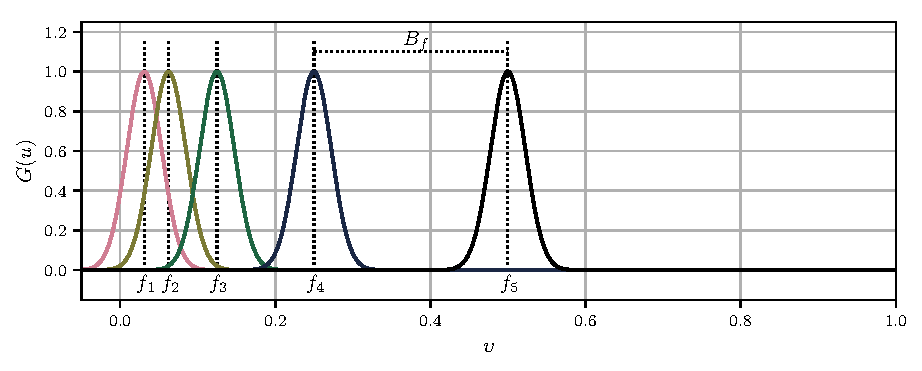
\includegraphics[width=\textwidth]{GaborFilterbank_freq_1d_octave_spacing.pdf}} \\
    \subcaptionbox{\label{fig:filterbnk_half_crossingpoint}}{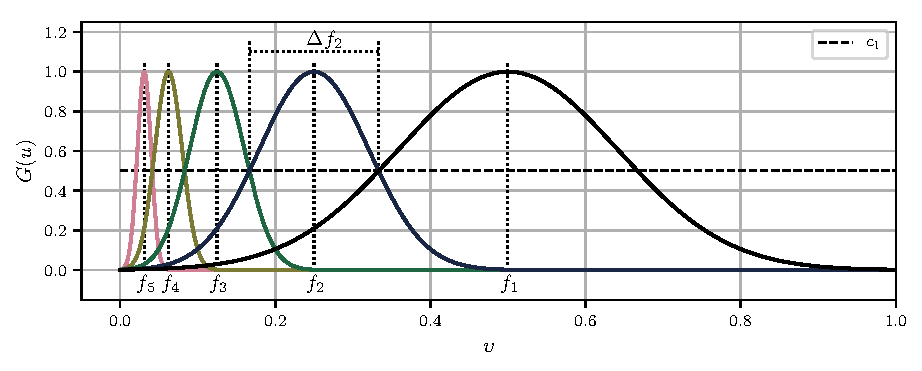
\includegraphics[width=\textwidth]{GaborFilterbank_freq_1d_half_crossingpoint.pdf}}\\
    \subcaptionbox{\label{fig:filterbnk_new_crossingpoint}}{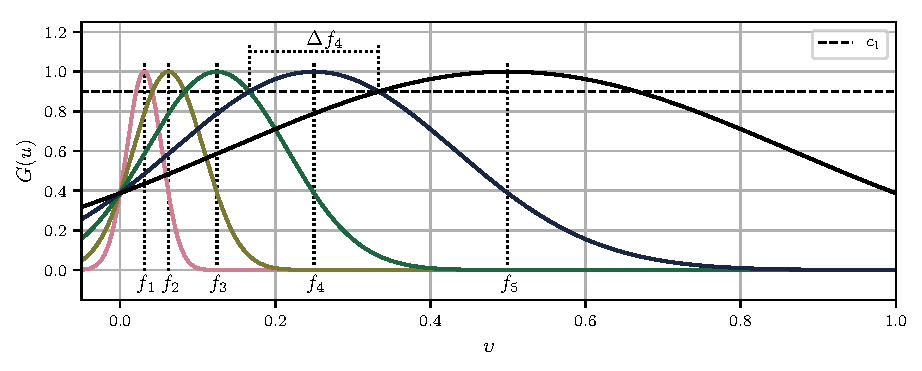
\includegraphics[width=\textwidth]{GaborFilterbank_freq_1d_new_crossingpoint.pdf}}
\caption{Filter spacing and crossing point effect represented on a bank of filters in the frequency domain: (a) Separation of filters in octaves without crossing point between adjacent filters $[B_f=1, \alpha=0.1, c_1=-]$, (b) High and low cut-off frequency points given by $\Delta f$ $[B_f=1, \alpha=f/\gamma, c_1=0.5]$, (c) Filter bank behavior after changing the crossing point $[B_f=1, \alpha=f/\gamma, c_1=0.9]$.}\label{fig:1d_filterbank_spacing}
\end{figure}

\subsection{2-d Gabor filters}

The generalization of the previously defined Gabor's function theory in 1-d to two dimensions is straightforward. First, we replace the time variable $t$ with the pair of spatial coordinates $(x, y)$ and the frequency variable $f$ with the pair of frequency variables $(u, v)$. Then, as for the 1-d case, the 2-d Gabor functions follows the Heinsenberg principle where the uncertainty measures for the space and spatial-frequency domains are expressed in terms of $\Delta x$, $\Delta y$, $\Delta u$, and $\Delta v$, for which it holds that

\begin{equation}\label{eq:uncertainty_principle_2d}
    \begin{gathered}
        \Delta x\Delta u \geq \frac{1}{4\pi}, \, \Delta y\Delta v \geq \frac{1}{4\pi} \\
        \Delta x \Delta y \Delta u \Delta v \geq \frac{1}{16\pi^2}
    \end{gathered}
\end{equation}

In case 2d, the Gabor function is represented by the modulated product of a harmonic oscillation on any spatial frequency and any orientation, represented by a complex exponential, with a pulse in the form of a probability function, represented by an elliptical Gaussian ellipse on any orientation. For simplicity, it can be assumed that the orientation of the Gaussian and the harmonic modulation are the same, therefore, applying the given simplifications, a compact form of the 2-d GEF in the space domain can be defined as

\begin{equation}\label{eq:gabor_function_2d_space_compact}
    \begin{gathered}
        g(x, r) =  e ^{-\left(\alpha^2 x_r^2 + \beta^2 y_r^2\right)} e ^{j 2 \pi f x_r } \\
        x_r = x \cos{\theta} + y \sin{\theta}\\
        y_r = -x \sin{\theta} + y \cos{\theta}
     \end{gathered}
\end{equation}
whereas the analytical expression for the 2-d GEF in the spatial-frequency domain is obtained from the Fourier transform of \eqref{eq:gabor_function_2d_space_compact}, $G(u, v) = \mathcal{F}\{g(x, y)\}$, and is given by 

\begin{equation}\label{eq:gabor_function_2d_frequency_compact}
    \begin{gathered}
        G(u, v) =  \frac{\pi}{\alpha \beta} e ^{- \pi^2 \left(\frac{\left( u_r - f\right)^2}{\alpha^2} + \frac{v_r^2}{\beta^2}\right)} \\
        u_r = u \cos{\theta} + v \sin{\theta}\\
        v_r = -u \sin{\theta} + v \cos{\theta}
     \end{gathered}
\end{equation}

The above expressions can be normalized by following the same reasoning as in the 1-d case. We apply the maximum value condition \eqref{eq:maximun_condition} and the constant spectrum condition \eqref{eq:constant_spectrum_condition} described in Section \ref{subsec:filter_normalization} to get $\max{|G(u,v)|} = 1$ and $\int_{-\infty}^{\infty} \int_{-\infty}^{\infty} |g(x,y)| dx dy = 1$ for a filter on any frequency $f$ and orientation $\theta$. 
Under these circumstances, the normalization constant is defined by

\begin{equation}\label{eq:normalization_constant_2d}
    \frac{\alpha \beta}{\pi}
\end{equation}
and the normalized Gabor function in both 2-d domains as 

\begin{equation}\label{eq:gabor_function_2d_spacefrequency_normalized}
    \begin{gathered}
        g(x, r) = \frac{\alpha \beta}{\pi} e ^{-\left(\alpha^2 x_r^2 + \beta^2 y_r^2\right)} e ^{j 2 \pi f x_r } \\
        G(u, v) =   e ^{- \pi^2 \left(\frac{\left( u_r - f\right)^2}{\alpha^2} + \frac{v_r^2}{\beta^2}\right)} 
     \end{gathered}
\end{equation}

\subsubsection{Orientation filter spacing}

The Gabor filter defined by equations \eqref{eq:gabor_function_2d_spacefrequency_normalized}, used to generate a in a filter bank at different frequencies and orientations, does not cover most of the spectrum, therefore it is not useful for the reconstruction of a signal and/or the extraction of features (see Figure \ref{fig:2d_filterbank_octave_spacing}). To obtain a more encompassing filter bank, it is evident that we need to include a relationship between the sharpness of the Gaussian window and the central frequency. 

The sharpness of the Gaussian function, unlike the 1-d case, now includes two variables ($\alpha, \beta$) that affect the effective width of the Gabor filter envelope. Such an envelope can have an elliptical shape, then $\alpha $ controls the length of the major axis while $\beta$ controls the length of the minor axis. 

The analysis of the frequency separation in octaves between adjacent filters of a bank carried out in the Section \ref{subsec:frequency_filter_spacing} is valid in the 2-d case. The full bandwidth of half the frequency response, $B_f$, represents the separation between the center frequencies; the interval $\Delta f$ represents the distance between the points where $G(u, v)$ begins to decrease and; the full frequency bandwidth through the ratio $\gamma$ and the crossing point $c_1$ allows adapting the size of the major axis of the envelope $\alpha$ depending on the center frequency $f$.

We can do a similar analysis for the minor axis of Gabor's envelope. First, notice that insertion of the orientation variable in the 2-d case, $\theta$, implies the existence of an angular separation $B_{\theta}$ between the centers of the filters in a bank (see Figure \ref{fig:2d_filterbank_octave_spacing}). This angular bandwidth can be defined by the number of orientations $N$ in the filter bank such that $B_{\theta} = \frac{\pi}{N}$. Then, we propose to vary the length of $\beta$ as a function of the central frequency and the angular bandwidth through the angular interval $\Delta \theta$, which is the distance along $\beta$ where $G(u, v)$ begins to decrease.

\begin{equation}\label{eq:orientation_interval_crossing_point}
    \frac{\Delta \theta}{2} = \frac{\beta}{\pi}\sqrt{\ln \left(\frac{1}{c_2}\right)}
\end{equation}

Then, we know that for a filter whose center frequency is $f$ and whose cut-off angular interval is $\Delta \theta$, the full orientation bandwidth expressed in radians, $B_\theta$, is defined as \cite{Daugman:JOSA:1985a}

\begin{equation}\label{eq:orientation_bandwidth_interval}
    B_{\theta} = 2 \tan^{-1} \left( \frac{\Delta \theta}{2f} \right)
\end{equation}

It is clear that using expression \eqref{eq:orientation_interval_crossing_point} in equation \eqref{eq:orientation_bandwidth_interval}, we find the expression that relates the frequency bandwidth to the central frequency and the length of the Gaussian minor axis.

\begin{equation}\label{eq:orientation_bandwidth}
    B_{\theta} = 2 \tan^{-1} \left( \frac{\beta}{\pi f} \sqrt{\ln \left(\frac{1}{c_2}\right)} \right)
\end{equation}

Taking the above relationships permits to write the 2-d GEF to use it into a bank as follows. 

\begin{equation}\label{eq:gabor_function_2d_spacefreq_bank}
    \begin{gathered}
         g(x,y) =  \frac{f^2}{\gamma \eta \pi} e ^{-\left(\frac{f^2}{\gamma^2} x_r^2 + \frac{f^2}{\eta^2} y_r^2\right)} e ^{j 2 \pi f x_r } \\
         G(u,v) =  e ^{-\left(\frac{\pi}{f}\right)^2\left( \gamma^2 (u_r-f)^2 + \eta^2 v_r^2\right)}
     \end{gathered}
\end{equation}
where now the length $\alpha$ of each filter in the bank will be determined based on the ratio $\gamma = \frac{f}{\alpha}$ and crossing point between adjacent filters $c_1$; and the length $\beta$ will be determined based on the ratio $\eta = \frac{f}{\beta}$ and crossing point between adjacent filters $c_2$.

The figure \ref{fig:2d_filterbank_spacing} shows the octave spacing and the orientation bandwidth for a bank of filters in the frequency domain. Particulary, the figure \ref{fig:2d_filterbank_octave_spacing} shows a bank without the relationship between the effective width and the central frequency of the filter, whereas the figures \ref{fig:filterbank_half_crossingpoint} show the interdependence between $\alpha$, $\beta$, $B_f$, $B_{\theta}$, $f$ and the crossing points $c_1$, $c_2$.

\begin{figure}
\centering
    \subcaptionbox{\label{fig:2d_filterbank_octave_spacing}}{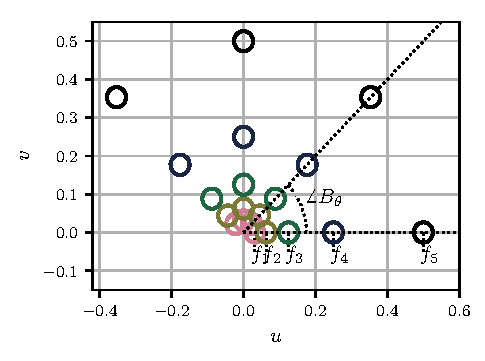
\includegraphics[width=0.49\textwidth]{GaborFilterbank_freq_2d_octave_spacing.pdf}}
    \subcaptionbox{\label{fig:2d_filterbank_half_crossingpoint}}{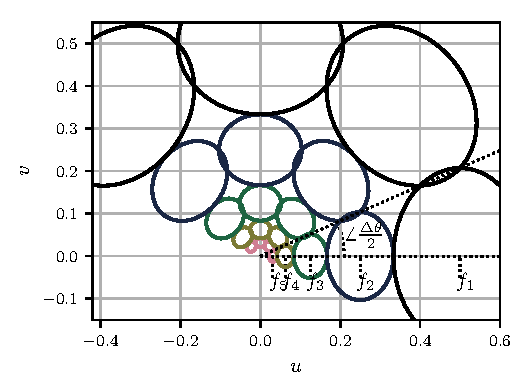
\includegraphics[width=0.49\textwidth]{GaborFilterbank_freq_2d_half_crossingpoint.pdf}}    
\caption{Filter spacing and crossing point effect represented on a bank of filters in the frequency domain: (a) Separation of 2-d filters without crossing points between adjacent filters $[B_f=1, B_{\theta} = 45^{\circ}, \alpha=\beta=0.1, c_1=c_2=-]$, (b) High and low cut-off frequency points given by $\Delta f$ and $\Delta \theta$ $[B_f=1, B_{\theta} = 45^{\circ}, \alpha=f/\gamma, \beta=f/\eta, c_1=c_2=0.5]$.}\label{fig:2d_filterbank_spacing}
\end{figure}

\section{Similarity Measure Apply on Texure Distribution}
\section{Partial Conclusions}